\documentclass[11pt]{article}
\usepackage[margin=1in]{geometry}
\usepackage{booktabs}
\usepackage{graphicx}
\usepackage{microtype}
\usepackage[hidelinks]{hyperref}

\newcommand{\rcLandmark}{0.742}
\newcommand{\rcPool}{0.85}
\newcommand{\rcSpine}{0.917}


\title{\vspace{-2em}\textbf{Subgraph retrieval quality}}
\author{arxivkg · retrieval · the committed recipe in isolation}
\date{}

\begin{document}
\maketitle
\vspace{-2em}

\section*{What we did}
The committed retrieval recipe --- hybrid pool (asym cosine $\cup$ title-BM25) $\rightarrow$
backward-ancestor augmentation $\rightarrow$ induce citation subgraph $\rightarrow$
Personalized-PageRank landmark ranking --- is locked; this measures the one thing it does:
recovering a field's \emph{canonical landmark papers} as a bounded, connected, on-topic citation
subgraph. \textbf{Retrieval level only: no LLM, no compose, no judge.} Over each gold topic we build
one shared candidate pool and run three Stage-4 selectors on it: \texttt{induce} (the committed
PPR), \texttt{pcst} (Prize-Collecting Steiner Tree, G-Retriever \href{https://arxiv.org/abs/2402.07630}{2402.07630}),
and \texttt{dsa\_bfs} (similarity-aware BFS, DynaGRAG \href{https://arxiv.org/abs/2412.18644}{2412.18644}).
Splitting \texttt{pool\_recall} (the reachability ceiling) from \texttt{landmark\_recall} (after
ranking) localizes any loss: a gap is a \emph{ranking} problem, a low ceiling a \emph{reach} problem.

\section*{Results (3 gold topics: diffusion, transformer, testtime)}
\begin{center}\begin{tabular}{lrrrrr}
\toprule
method & pool rec. & landmark rec. & spine rec. & conn. & cosine \\
\midrule
induce (committed) & 0.85 & 0.742 & 0.917 & 0.908 & 0.497 \\
pcst & 0.85 & 0.397 & 0.483 & 1.0 & 0.602 \\
dsa\_bfs & 0.85 & 0.467 & 0.6 & 0.975 & 0.577 \\
\bottomrule
\end{tabular}
\end{center}
\begin{center}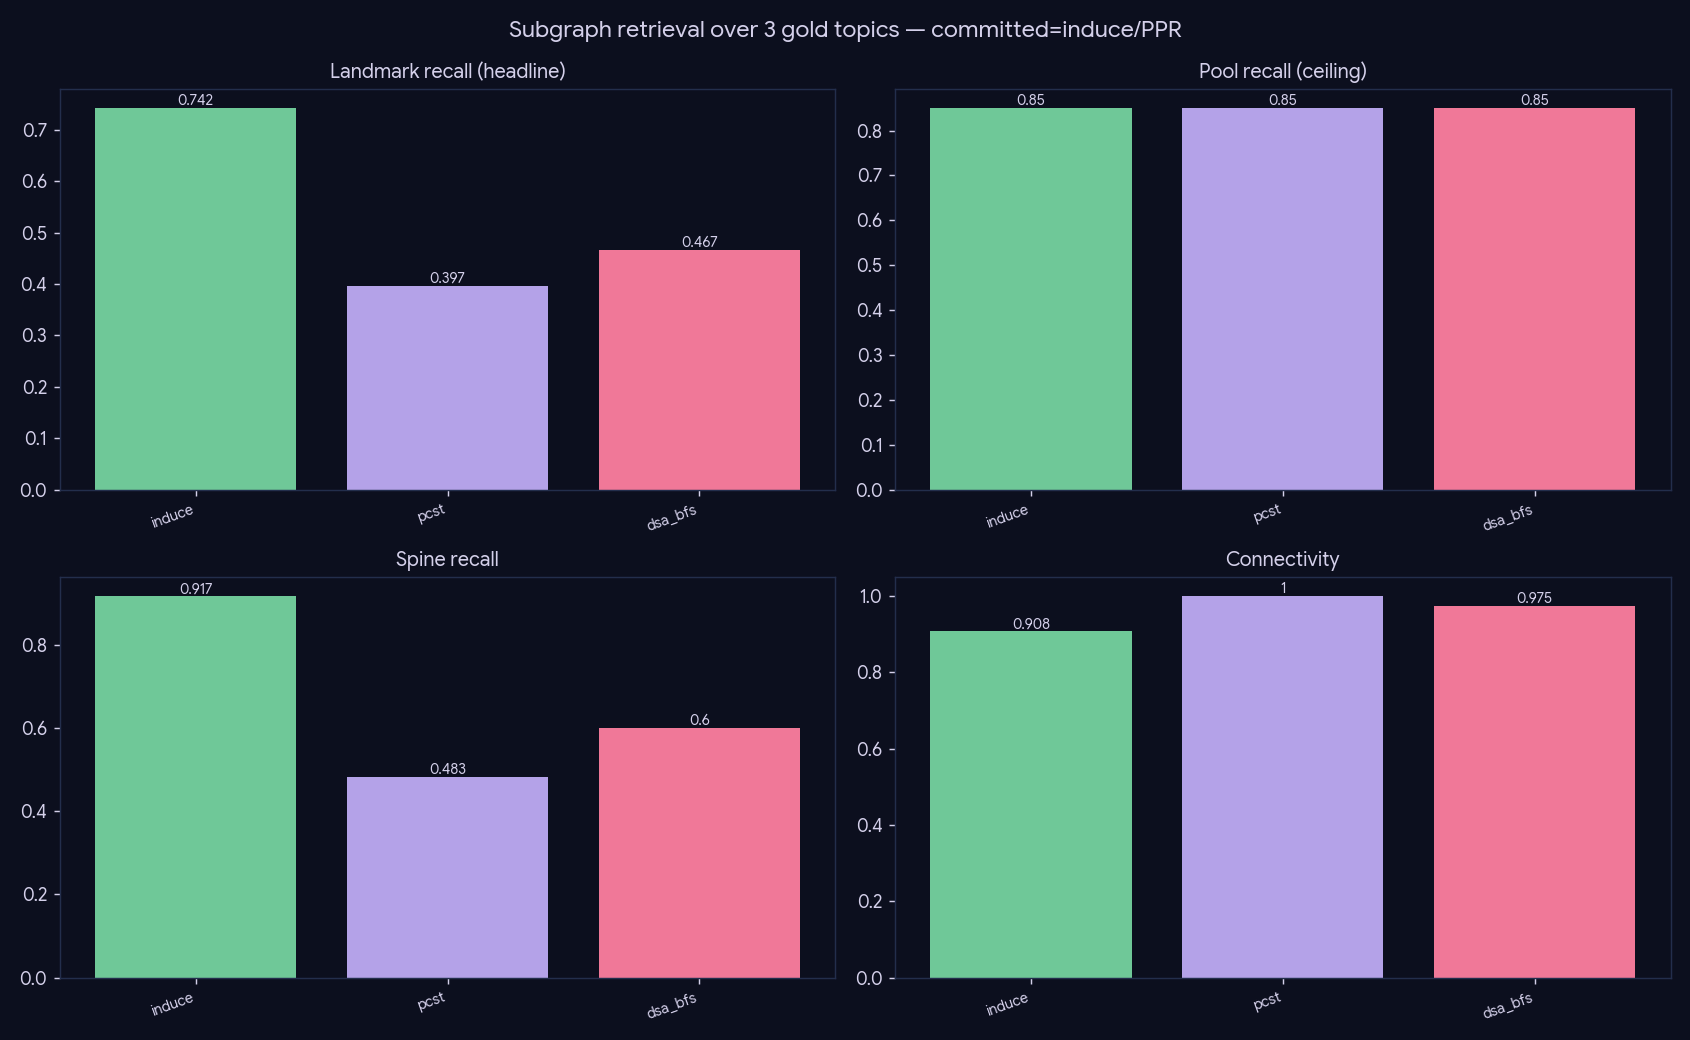
\includegraphics[width=0.95\textwidth]{../results/ablation.png}\end{center}

\section*{Conclusion}
\textbf{The committed \texttt{induce}/PPR method recovers \rcLandmark{} of canonical landmarks and
\rcSpine{} of the foundational spine}, against a shared pool ceiling of \rcPool{} --- so PPR ranking
retains $\rcLandmark/\rcPool \approx 87\%$ of everything reachable, and almost the entire origin
story. The $0.85$ ceiling (not $1.0$) is a pool-\emph{reach} limit, not a ranking flaw: the missing
canonical papers fall outside the topical cosine cloud or are uncited within it --- a candidate-pool
question (wider \texttt{n\_pool} / more ancestor hops), not a selector one. \textbf{\texttt{induce}
dominates every recall axis.} \texttt{pcst} wins \emph{only} connectivity ($1.0$) and mean-cosine
while \emph{halving} landmark recall ($0.40$) --- its cosine prize $\neq$ citation centrality, so it
keeps tight high-cosine clusters and drops central-but-not-top-cosine canonical papers. Membership
must be decided by PPR; connectivity is a downstream \emph{presentation} concern (the lineage tree
adds Steiner bridges \emph{over} the PPR landmarks, buying PCST-level connectivity without its recall
cost). \textbf{Caveat:} n$=3$ (the only topics with curated gold); per-topic numbers are stable
(\texttt{induce} landmark\_recall $=0.625/0.60/1.0$), but a wider gold battery is the cheapest way to
harden the claim.

\end{document}
